\section{Product perspective}
\subsection{Class Diagrams}
The diagram below represents and describes the classes involved in the system, their functionalities and how they interact.

\begin{figure}[ht]
    \centering
    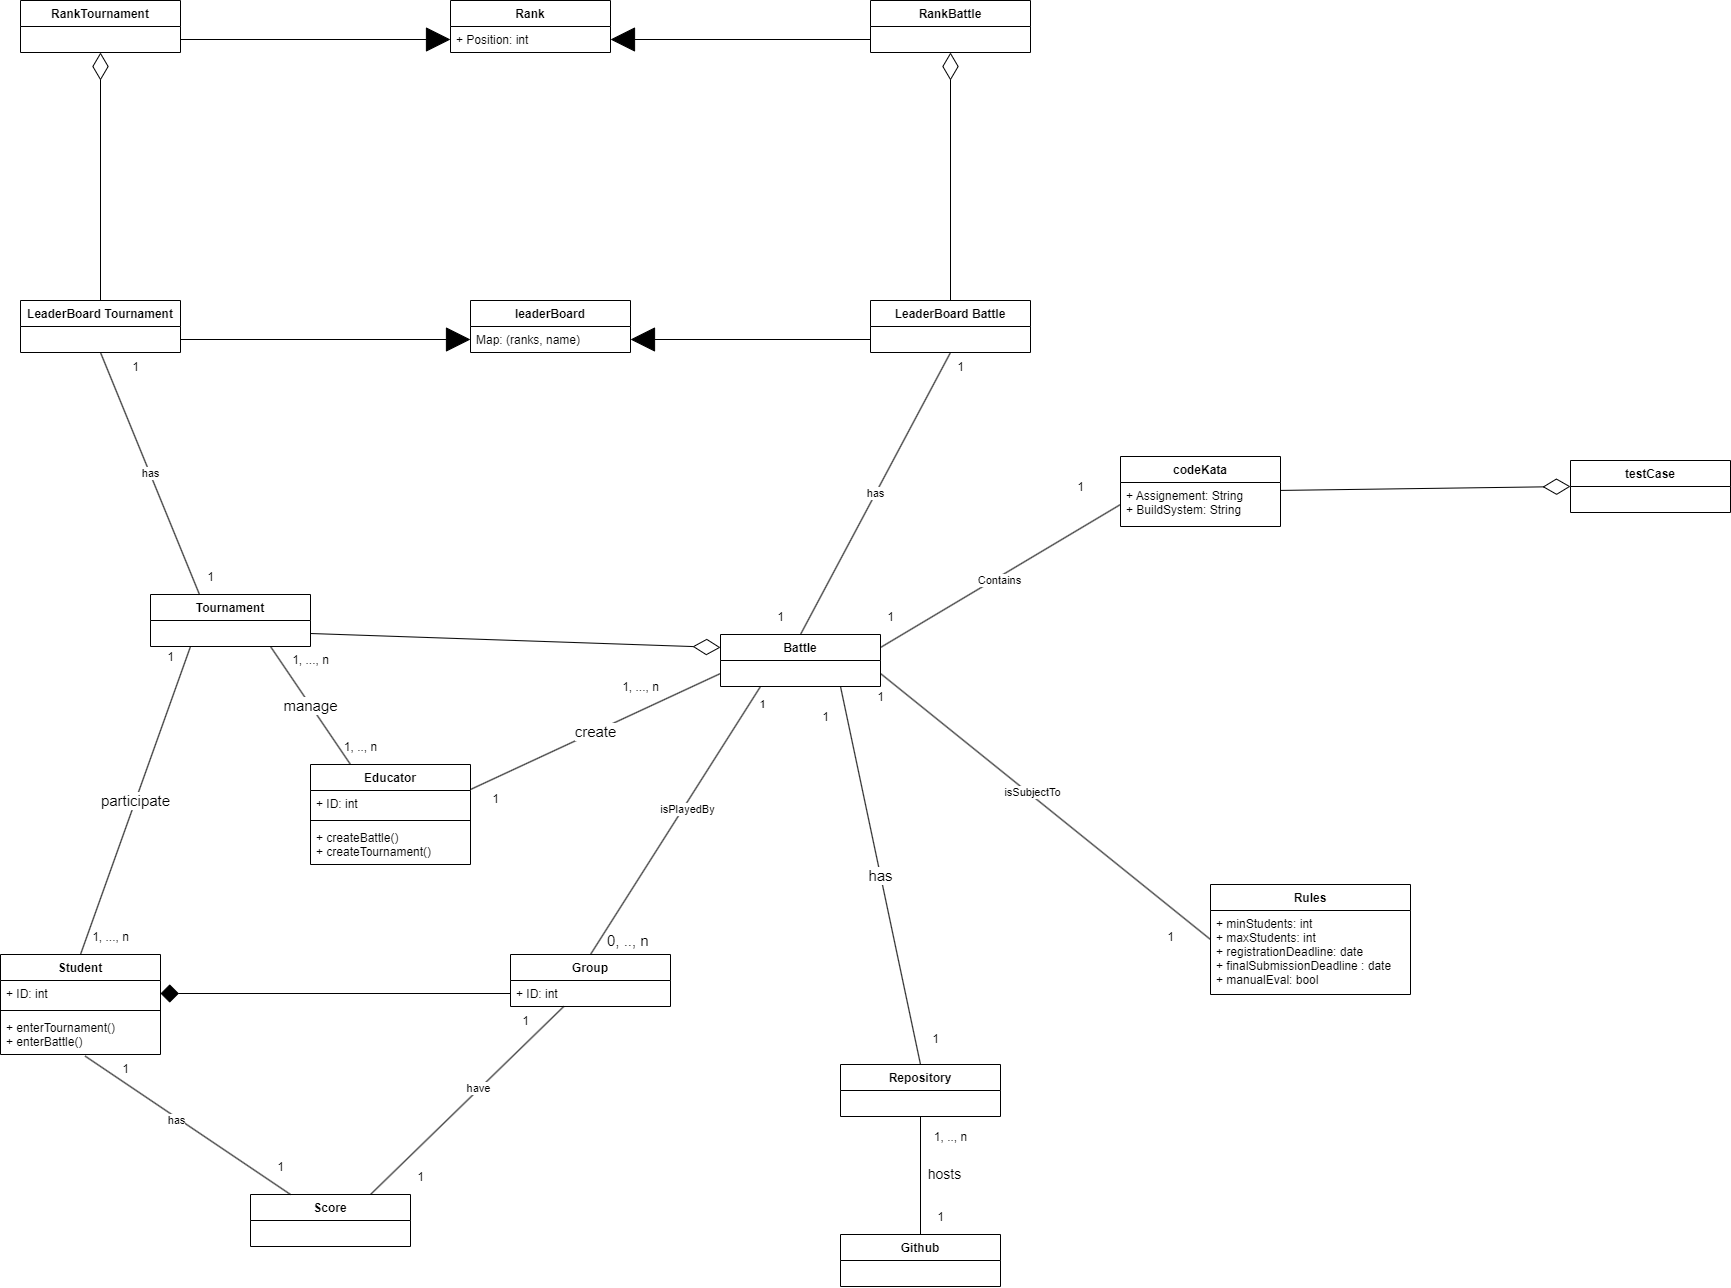
\includegraphics[width=1\linewidth]{misc//Images/classDiagram.png}
    \caption{Class Diagram}
    \label{fig:enter-label}
\end{figure}



\subsection{Scenarios}
\begin{enumerate}
    \item \textbf{User signs into platform}\newline
    Professor Layton wants to evaluate the performance of his programming students but he has no easy way to do so. Fortunately he knows about \ac{CKB} that can allow him to write a few coding challenges and automatically score his students submissions. He reaches the platform and is presented with a Sign In page where he has to full fill his details and set his profile to educator.\newline Luke is a student of Professor Layton and when he heard that the professor is using \ac{CKB} he immediately reached it and signed up by full filling his details and setting his profile to student.
    
    \item \textbf{User logs into platform}\newline
    A student that want to access the functionalities of the platform can log in , an educator does the same.
    
    
    \item \textbf{Educator creates tournament}\newline
    Professor Layton, now signed into \ac{CKB}, can create a new tournament and add collaborators to it. Once the tournament has been created every user subscribed to the \ac{CKB} platform is notified and can enter it.
    
    \item \textbf{Educator creates battle}\newline
    An educator wants to add another battle in the context of a tournament he is partecipating in. 
    He starts by creating a \ac{CK} assignment (containing description, software project, test cases and build automation scripts) and ultimately creates the battle using the \ac{CKB} platform.  
    On the \ac{CKB} platform the educator then uploads the \ac{CK} assignment and sets:
    \begin{itemize}
        \item minimum and maximum number of students per group,
        \item set a registration deadline,
        \item set a final submission deadline,
        \item set additional configurations for optional manual scoring 
    \end{itemize}
    
    Once the battle in is created all the students subscribed to the tournament of said battle receive a notification of its creation.
    
    \item \textbf{Student subscribes to a tournament}\newline
    Once a student is logged into the website he is presented with a list of available tournaments he can join. By clicking on one of them the tournament description will be available for him to read and if he wants he can click on join to take part in that tournament.
    
    \item \textbf{Student joins a team for a battle}\newline
    The students are notified of a new battle in the context of a tournament.
    A student that decides to join the battle may be asked to join as a group (in case the battle rules ask for it ), and so he invites other students using the \ac{CKB} platform to create a group that respects the group dimension rule.  
    Once every student accepts the new group joins the battle.   
    
    Once the subscription deadline expires the \ac{CKB} platform creates a GitHub repository containing the \ac{CK} and sends every student a link for it.  
    At this point for every group the students fork the repository and set up the automated workflow with Github Actions.
    At this point the group is ready to start working on the \ac{CK}.
    
    
    \item \textbf{Application scores a commit from a student}\newline
    Every time a student commits some work to the forked repository the platform is notified and starts to run its automated evaluation by pulling the sources and running tests for:
    \begin{itemize}
        \item functional aspects, measured in terms of number of test cases that pass out of all test cases;
        \item timeliness, measured in terms of time passed between the registration deadline and the last commit;
        \item quality level of sources, extracted through static analysis tools.
    \end{itemize}
    
    \item \textbf{Users look at current battle ranks}\newline
    At any point the students that joined a battle and the educators that are involved with it are able to look at the ranking for said battle. Every group position is determined by the score given by the platform to their solution of the \ac{CK}.
    
    \item \textbf{Battle submission deadline expires}\newline
    When the submission deadline expires the battle goes into a consolidation stage where, if decided at the creation, educators can manually assign scores to each team by inspecting sources. Once this stage has ended all students participating in the battle are notified about their final battle rank and the tournament score is updated.
    
    \item \textbf{Educator closes tournament}\newline
    At some point an educator decides that it is time to close a tournament, which he does through the platform. Then, as soon as the final tournament rank is available, \ac{CKB} platform notifies all the students that were subscribed to the tournament that it has ended.
 
    
    \item \textbf{Users look at tournament ranks}\newline
    Between battles and after the end of a tournament users can look at the tournament leader board. The position of every student is determined by the sum of all battle scores.
    
\end{enumerate}

\newpage
\section{Product functions}
\textbf{An Educator Creates a Tournament}\newline
The main functionality of \ac{CKB} is to offer Educators the possibility of creating tournaments and battles inside of them. An Educator can decide to also add collaborators to the tournament, in order to ease the managing of it all.
\textbf{A Student joins a Tournament}\newline
\ac{CKB} offers the possibility to Students to join any tournament they like and to partecipate to as many as they want. Inside a tournament students can then join battles in a group and climb its leader-boards.

\section{User characteristics}
The actors listed below are considered in the \ac{CKB} system:\newline
\begin{itemize}
    \item Student: User that participates in tournaments and battles. He/She can subscribe to new tournaments and join battles alone or in team;
    \item Educator: User that managed tournaments and battles. He/She can create and end tournaments and add new battles to the created tournaments;
    \item GitHub: Another platform used by the \ac{CKB} system to create and manage code repositories.
\end{itemize}

\section{Assumptions, dependencies and constraints}
\begin{center}
    \begin{longtable}{ |l|p{0.9\linewidth}| }
        \hline
        \textbf{ID} & \textbf{Description}\\
        \hline
        A1 & The students can correctly setup the Github actions workflow. \\
        \hline
        A2 & An educator will complete the manual evaluation \\
        \hline
        A3 & Github will always notifies the CKB platform after every student commit \\
        \hline
        A4 & Students are always able to create a group to join a battle \\
        \hline
        A5 & Educators will only close a tournament when no battle is still ongoing\\
        \hline
        A6 & Only the Educator who created the tournament will close it\\
        \hline
    \end{longtable}
\end{center}